\documentclass[11pt]{article}

\usepackage{common}
\title{Practical 4: Reinforcement Learning}
\author{Lisa Lu (lisalu@college.harvard.edu) \\ Matt Leifer (matthewleifer@college.harvard.edu) \\ Janet Chen (janetchen@college.harvard.edu) }

\begin{document}
\maketitle
\section{Technical Approach}

We chose to approach this problem with Q-Learning: online updates and greedy actions, which we modified to include an epsilon-greedy approach that would choose the maximal greedy action $\epsilon$ of the time and explore $1-\epsilon$ of the time.

The most challenging aspect of this problem was the extremely large state space: if we had used pixels as our states, it is unlikely that our values and policy would have converged in the few-dozen rounds of training allowed. To address this, we tried several methods of discretizing the state space. We first tried binning the screen locations uniformly: 10 bins of 60 pixels each for the horizontal direction and 10 bins of 40 pixels each for the vertical direction. Unfortunately, this approach led to little success-- our scores never exceeded $\approx2$, even after much experimentation with different $\eta, \gamma,$ and $\epsilon$ values. 

We then came across an article at tonypoer.io (see References) that suggested using non-uniform bins: in particular, more small bins for areas close to the trees and fewer large bins for areas far from the trees. This made sense to us, since timing of jumps is more crucial for actions taken closer to the trees. For example, jumping at 400 vs 410 pixels away from the tree won't affect the monkey's collision likelihood as much as jumping 10 vs 20 pixels away from the tree. Ultimately, however, though we experimented with a variety of bin quantities and bin sizes, we were unable to find an arrangement that beat a uniform 24x15 binning strategy. If we had more time, we would continue to try different distributions of non-uniform bins. 

Our first major breakthrough was to infer the value of gravity and factor that into our state space. We did this using the following method:
\begin{enumerate}
	\item In every instance, don't jump in the first time step
	\item Check the monkey's velocity in the second time step to infer gravity. Since $v_0 = 0$, $v_1 = 0 - g$ and $g = - v_1$.
\end{enumerate}

To factor gravity into our model, we doubled the state space to be (horizontal distance) x (vertical distance) x (gravity), where $|\text{horizontal distance}| = 15, |\text{vertical distance}| = 24, |\text{gravity}| = 2$. When we factored gravity into the state space, we achieved three-digit maximum scores and two-digit average scores after 150 epochs of training. In a later table, one trial had a max score of 106, but the average score was still low (~5), so we knew we had to keep tuning our strategy, though gravity clearly made a big improvement on our agent.

Another optimization was to add velocity to the state space via one bin for positive velocities and one bin for negative velocities. This made intuitive sense, since, all else constant, approaching a tree with negative velocity required very different actions than does approaching with positive velocity.

We also used decreasing schedules for the learning rate $\eta$ and greedy rate $1-\epsilon$ based on the number of iterations. This allowed us to be more greedy as we became more confident in our model of the world, shifting away from exploration towards exploitation and maximizing reward.  We tried various other ways to decrement $\eta$ and $\epsilon$ as the iterations progressed but the most successful method we found was to set $\eta$ and $\epsilon$ to be inversely proportional to the iteration we were on.  We tuned the discount factor, $\gamma$, to optimize our results. 

\section{Results}
This table shows our results using various different strategies, trained on 150 epochs.  Our final best strategy incorporated uniform binning of horizontal and vertical distances, two bins for velocity (positive and negative), two bins for the two possible gravity values, and decreasing schedules for epsilon and the learning rate based on the number of iterations. \normalsize
\\\\
\begin{tabular}{c|c|c}
Strategy & Average Score & Max Score \\ 
\hline
Random (stub code) & 0.14 & 1 \\ 
Uniform bins (15x24) & 5.593333333 & 106 \\ 
Non-Uniform bins (15x24), g. $\eta$ = 0.7, $\gamma$ = 1, $\epsilon$ = 0.9 & 2.35 & 27 \\ 
Non-Uniform bins (10x10), g., velocity, $\eta$ = 0.7, $\gamma$ = 1, $\epsilon$ = 0.9 & 3.25 & 27 \\ 
$\epsilon$ Schedule & 1.213333333 & 17 \\ 
Velocity & 15.52 & 190 \\ 
Learning Schedule (visited) & 3.366666667 & 75 \\ 
Learning Schedule (iter) & 12.84666667 & 219
\end{tabular}
\\\\\\
For each trial, the strategy was run for 150, as well as 1000, epochs. We did not expect convergence/decent results in a few dozen epochs as claimed in the practical specification because previous versions of this practical had a fixed gravity constant. Since gravity played a large role in this game and essentially quadrupled our state space by affecting both gravity and velocity, we expected decent results in quadruple the number of a few dozen epochs.

For 1000 epochs, these were our results for tuning various values of the discount factor, $\gamma$.  If we look longterm and compare these results to the ones with fewer trials they do perform better on average, but as the graph below shows, there is still a significant amount of variability in how well the monkey does, though he does consistently make it into double digit scores.  
\\\\
\begin{tabular}{c|c|c|c|c|c}
$\gamma$ & Avg. & Avg.-4 & Avg.-1 & Max-4 & Max-1 \\
\hline
0 & 1.248 & 0.488 & 2.045 & 13 & 20 \\ 
0.1 & 28.385 & 56.206 & 0.453 & 624 & 5 \\ 
0.2 & 35.188 & 66.449 & 0.498 & 893 & 3 \\ 
0.3 & 37.584 & 75.772 & 0.598 & 748 & 3 \\ 
0.4 & 20.205 & 39.86 & 0.55 & 479 & 4 \\ 
0.5 & 48.854 & 99.979 & 0.707 & 1461 & 4 \\ 
0.6 & 56.429 & 110.434 & 0.890 & 1338 & 6 \\
0.7 & 49.851 & 97.746 & 0.596 & 1011 & 3 \\ 
0.8 & 52.916 & 104.833 & 0.582 & 824 & 5 \\ 
0.9 & 57.917 & 110.107 & 0.464 & 973 & 3 \\ 
1 & 34.987 & 69.623 & 0.489 & 878 & 3
\end{tabular} 
\\
\\
Avg.-4 gives the average score for epochs that had gravity equal to 4 and likewise for avg.-1, max-4, and max-1.  Max-4 is the maximum value over all the trials in a 1000 epoch period that had trials that was mixed with gravity that was 4 and gravity that was 1. 
\\
\\
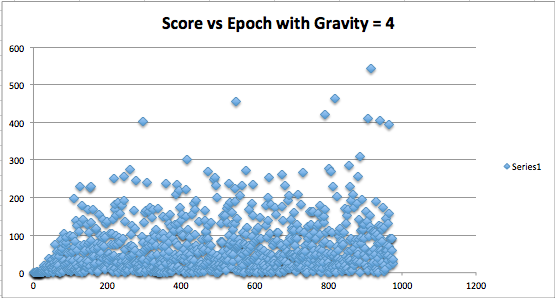
\includegraphics[scale=0.8]{G_4_Graph.png} \\\\
This is a scatter plot of trials that had gravity equal to 4 over a trial of 2000 epochs.  The maximum value here is 542 and the average score for any epoch here is 65.9.  You can clearly see that at the very beginning it learns quickly and by the 80th epoch it's cracked a score of 100.  
\section{Discussion} 

We decided to spend the majority of our time finding a good state space. The first major challenge here was finding a computationally tractable representation of the pixels in the world. Although there were many pixels, we thought that binning pixels with nearby neighbors would allow for sufficient accuracy to jump through the gaps. We first tried naive uniform binning (which was the approach we ended up sticking with) and then binning with higher density near the gaps. Although we were unable to find a non-uniform binning arrangement that improved performance in the time provided, this approach made intuitive sense to us and was supported by our outside research. Because of this, we think that non-uniform binning did not work for us mostly because we did not define suitable bins.

After we found a decent representation of the pixels, we decided to add a gravity dimension to our state space. This drastically improved our performance, which makes sense: gravity has a major effect on how productive the monkey's jumps are.

After seeing how much adding gravity to the state space improved the monkey's performance, we wanted to continue exploring other factors affected by gravity and landed on velocity. We added 2 velocity bins to the state space, one for positive velocities and one for negative. This improved our monkey's performance event more, likely because whether the monkey is traveling up or down affects whether it should jump.

Perhaps the greatest predictor of how many epochs it would take for the monkey to start performing well was how early its early successful trial appeared. If it got lucky early on and found a successful strategy early on (one that gave it a score of say 30 or more) the rest of the trial would be far more successful.  If the monkey got lucky each individual trial would be longer it would have more time to learn how to play the game per epoch, so using the number of epochs can be a somewhat misleading metric.

Additionally, it is worth noting that our monkey performed better when gravity = 4 than when gravity = 1. This is because when gravity = 4, it dominated the noisiness of impulse, making overall velocity much more predictable. However, when gravity = 1, the noise of the impulse had much more relative weight and our monkey performed worse. Having the gravity dimension of the problem also caused our model to take longer than a couple dozen epochs to converge: with 2 possible gravity values, our state space was twice as large, and therefore we expected it to take twice as long on average to converge.

\section{References}
https://tonypoer.io/2016/12/15/making-an-ai-to-play-flappy-bird-w-q-learning/
\end{document}
